\documentclass[tikz,border=4pt]{standalone}
\usepackage{amsmath}
\usepackage{xcolor}
\usepackage{xspace}
\usepackage{tikz}
\usetikzlibrary{arrows.meta,positioning}

\definecolor{caraprimary}{RGB}{30,60,120}
\definecolor{caraaccent}{RGB}{200,80,60}
\newcommand{\effnet}{EfficientNet-B0\xspace}

\begin{document}
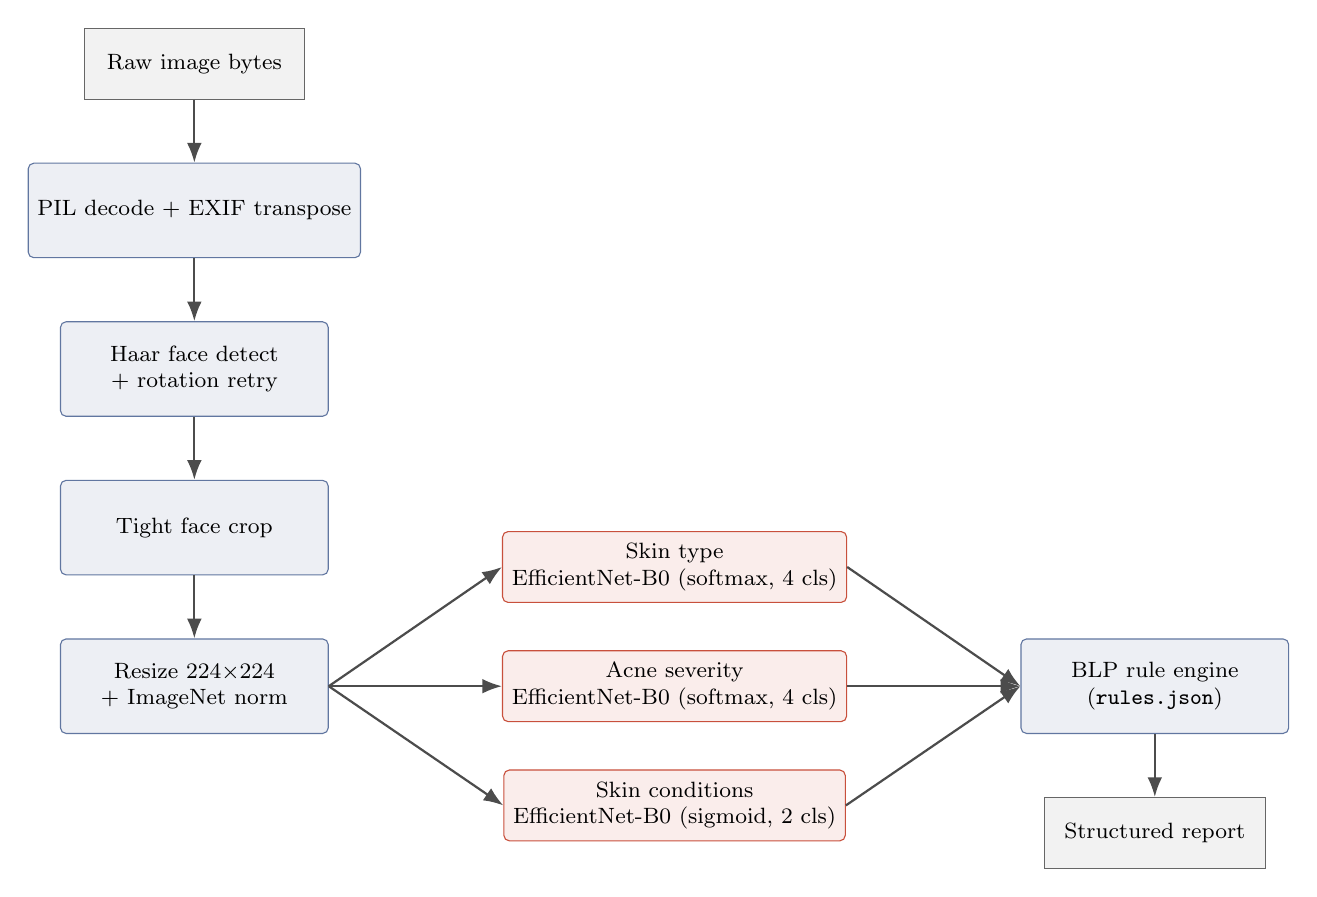
\begin{tikzpicture}[
    node distance=8mm,
    every node/.style={font=\footnotesize},
    stage/.style={rectangle, draw=caraprimary!70, fill=caraprimary!8,
        minimum height=1.2cm, minimum width=3.4cm, rounded corners=2pt,
        align=center},
    data/.style={rectangle, draw=black!60, fill=black!5,
        minimum height=0.9cm, minimum width=2.8cm, align=center},
    model/.style={rectangle, draw=caraaccent, fill=caraaccent!10,
        minimum height=0.9cm, minimum width=3.4cm, rounded corners=2pt,
        align=center},
    arrow/.style={-{Latex[length=2.5mm]}, thick, draw=black!70}]

    \node[data]                       (raw)   {Raw image bytes};
    \node[stage, below=of raw]        (decode){PIL decode + EXIF transpose};
    \node[stage, below=of decode]     (detect){Haar face detect\\+ rotation retry};
    \node[stage, below=of detect]     (crop)  {Tight face crop};
    \node[stage, below=of crop]       (tens)  {Resize 224\(\times\)224\\+ ImageNet norm};

    \node[model, right=22mm of tens]  (acne)  {Acne severity\\\effnet (softmax, 4 cls)};
    \node[model, above=6mm of acne]   (skin)  {Skin type\\\effnet (softmax, 4 cls)};
    \node[model, below=6mm of acne]   (cond)  {Skin conditions\\\effnet (sigmoid, 2 cls)};

    \node[stage, right=22mm of acne]  (blp)   {BLP rule engine\\(\texttt{rules.json})};
    \node[data,  below=of blp]        (rep)   {Structured report};

    \draw[arrow] (raw)   -- (decode);
    \draw[arrow] (decode) -- (detect);
    \draw[arrow] (detect) -- (crop);
    \draw[arrow] (crop)   -- (tens);
    \draw[arrow] (tens.east) -- (skin.west);
    \draw[arrow] (tens.east) -- (acne.west);
    \draw[arrow] (tens.east) -- (cond.west);
    \draw[arrow] (skin.east) -- (blp.west);
    \draw[arrow] (acne.east) -- (blp.west);
    \draw[arrow] (cond.east) -- (blp.west);
    \draw[arrow] (blp)    -- (rep);
\end{tikzpicture}
\end{document}
